% !TEX root = Projektdokumentation.tex
\section{Beispiel 3}
\label{sec:beispiel3}

\subsection{Ausgangssituation} 
\label{sec:ausgangssituation3}
Wie in Abschnitt \ref{sec:voraussetzungen} beschrieben, liefert die Schulze Methode auch Ergebnisse, wenn Kandidaten gleich bewertet wurden oder nicht bewertet wurden. Nicht bewertete Kandidaten werden dabei behandelt, als wären sie alle vom Wähler auf dem letzten Platz gewählt worden, sodass jeder Kandidat, der vom Wähler bewertet wurde, den nicht bewerteten Kandidaten vorgezogen wird.

\begin{description}
\centering
\item[6 mal] $a \succ_{v} b \succ_{v} c \succ_{v}d$
\item[8 mal] $a \approx_{v} b \succ_{v} c \approx_{v}d$
\item[8 mal] $a \approx_{v} c \succ_{v} b \approx_{v}d$
\item[18 mal] $a \approx_{v} c \succ_{v} d \succ_{v}b$
\item[8 mal] $a \approx_{v} c \approx_{v} d \succ_{v}d$
\item[40 mal] $b \succ_{v} a \approx_{v} c \approx_{v}d$
\item[4 mal] $c \succ_{v} b \succ_{v} d \succ_{v}a$
\item[9 mal] $c \succ_{v} d \succ_{v} a \succ_{v}b$
\item[8 mal] $c \approx_{v} d \succ_{v} a \approx_{v}b$
\item[14 mal] $d \succ_{v} a \succ_{v} b \succ_{v}c$
\item[11 mal] $d \succ_{v} b \succ_{v} c \succ_{v}a$
\item[4 mal] $d \succ_{v} c \succ_{v} a \succ_{v}b$
\end{description}

Zur erläuterung betrachten wir einmal die Wahl $a \approx_{v} b \succ_{v} c \approx_{v}d$. Hier hat der Kandidat gesagt er möchte lieber Kandidat $a$ oder $b$ welcher ist ihm dabei egal, aber lieber einen von den Kandidaten als die Kandidaten $b$ oder $d$. Dort macht der Wähler aber auch kein Unterschied ob $b$ oder $d$ beide findet er gleich gut/schlecht.

\subsection{Lösungsschritte} 
\label{sec:loesungen3}
Nun muss man als nächstes wieder die Menge $N$ bestimmen, in den man die Kandidaten gegeneinander antreten lässt nur kann es diesmal zu Duellen ohne Sieger kommen, da beide gleich bewertet wurden. Diese Duelle werden dann nicht Berücksichtigt. 

Exemplarisch wird in Tabelle \ref{beispiel3ab} das Duell von Kandidat $a$ gegen Kandidat $b$ dargestellt. 

% !TEX root = Projektdokumentation.tex

\begin{longtable}[c]{|l|l|l|l|}
\hline
Duelle & $a$  & $b$  & Sieger \\ \hline
\endfirsthead
%
\endhead
%
1      & 6  &    & $a$      \\ \hline
\rowcolor[HTML]{9B9B9B} 
2      & 8  & 8  & keiner \\ \hline
3      & 8  &    & $a$      \\ \hline
4      & 18 &    & $a$     \\ \hline
5      & 8  &    & $a$    \\ \hline
6      &    & 40 & $b$    \\ \hline
7      &    & 4  & $b$     \\ \hline
8      & 9  &    & $a$    \\ \hline
\rowcolor[HTML]{9B9B9B} 
9      & 8  & 8  & keiner \\ \hline
10     & 14 &    & $a$    \\ \hline
11     &    & 11 & $b$    \\ \hline
12     & 4  &    & $a$    \\ \hline
Summe  & 67 & 55 &        \\ \hline
\caption{Duell $a$ gegen $b$, graue Felder sind nicht bewertet, da unentschieden (Beispiel 3)}
\label{beispiel3ab}\\
\end{longtable}


Wenn man dieses Verfahren für alle Kandidaten anwendet erhält man die Menge $N$ die in Tabelle \ref{beispiel3N} aufgetragen ist.

% !TEX root = Projektdokumentation.tex

\begin{longtable}[c]{|l|l|l|l|l|}
\hline
            & N{[}*,a{]} & N{[}*,b{]} & N{[}*,c{]} & N{[}*,d{]} \\ \hline
\endfirsthead
%
\endhead
%
N{[}a, *{]} & ---        & 67         & 28         & 40         \\ \hline
N{[}b, *{]} & 55         & ---        & 79         & 58         \\ \hline
N{[}c, *{]} & 36         & 59         & ---        & 45         \\ \hline
N{[}d, *{]} & 50         & 72         & 29         & ---        \\ \hline
\caption{Die Menge $N$ (Beispiel 3)}
\label{beispiel3N}\\
\end{longtable}

In Abbildung \ref{fig:graph3} sieht man den Graphen, der aus der Menge $N$ gebildet wurde, er sieht etwas anders aus als in Beispiel 1 und Beispiel 2, da wir hier nicht nur den Wert brachen von Kandidat $a$ nach Kandidat $b$, sondern auch den umgekehrten Weg von $b$ nach $a$. Die Werte müssen so gelesen werden, dass der erste Wert, der größere, den Sieg des Kandidaten gegen den Kandidaten auf dem die Pfeilspitze zeigt, darstellt.

\begin{figure}[!h]
\centering
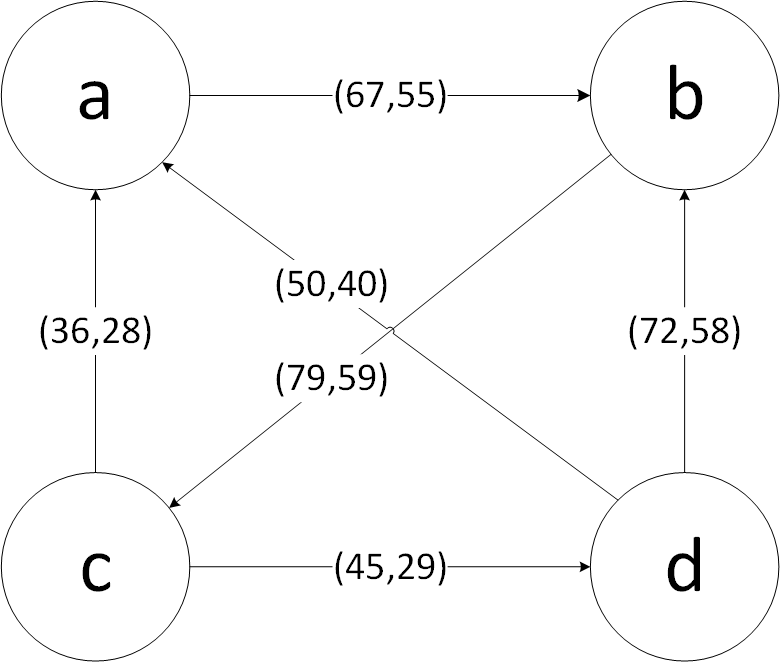
\includegraphics[scale=0.5]{Bilder/Beispiel3_Graph.png}
\caption{Graph über die Menge $N$(Beispiel 3)}
\label{fig:graph3}
\end{figure}

Nun gibt es vier Möglichkeiten einen Gewinner mit der \schulze zu finden. Wenn alle Wähler die Kandidaten in eine strikte Order gebracht haben, dann geben diese Methoden immer das selbe Ergebnis. Dieses Beispiel ist so aufgebaut, dass jede Methode einen anderen Kandidaten als Sieger ausgibt. Daher ist es wichtig vor der Wahl zu definieren, welche Wahlmethode genutzt wird.

\subsubsection[a]{margin}
\label{sec:margin}
Beim Ansatz $margin$ gewinnt der Kandidat, der seinen Sieg mit einem größeren Abstand erreicht. 
Untersucht wir Beispielhaft das Duell $a$ gegen $b$. Der Stärkste Weg von $a$ nach $b$, ist die direkt Verbindung, Kandidat $a$ erhält 67 Stimmen und Kandidat $b$ nur 55 Stimmen und damit gewinnt Kandidat $a$ mit 12 Stimmen Vorsprung. 
Aber auch Kandidat $b$ kann Kandidat $a$ schlagen, der Stärkste Weg für dieses Duell ist von $b$ über $c$ und $d$ nach $a$. Die schwächste Verbindung in diesem Weg ist die Verbindung $d$ nach $a$, da dort mit nur 10 Stimmen Vorsprung der Kandidat $d$, Kandidat $a$ schlägt.
Um den Gewinner Festzustellen vergleicht man nun den Abstand für den Sieg von $a$ (12 Stimmen)mit dem Sieg von $b$ (10 Stimmen) und erhält damit den Gewinner dieses Duells $a$.

Auch hier wurde in Tabelle \ref{beispiel3margin_p} die Menge $P$ aufgestellt. Die werte in der Tabelle zeigen nun den Abstand, mit dem der Kandidat den Gegner geschlagen hat.

% !TEX root = ../Projektdokumentation.tex
\begin{longtable}[c]{|l|l|l|l|l|}
\hline
            & P{[}*,a{]} & P{[}*,b{]} & P{[}*,c{]} & P{[}*,d{]} \\ \hline
\endfirsthead
%
\endhead
%
P{[}a, *{]} & ---        & 12         & 12         & 12         \\ \hline
P{[}b, *{]} & 10         & ---        & 20         & 16         \\ \hline
P{[}c, *{]} & 10         & 14         & ---        & 16         \\ \hline
P{[}d, *{]} & 10         & 14         & 14         & ---        \\ \hline
\caption{Die Menge $P$ nach margin Regel(Beispiel 3)}
\label{beispiel3margin_p}\\
\end{longtable}

Anschließend wird mit den Werten der Menge $P$ die neu Zweikampfsituation erstellt und man erhält die Relation $\mathcal{O}_{margin} = \{ ab, ac,ad,bc,bd,cd \}$

Daraus ergibt sich die Ergebnismenge $\mathcal{S}_{margin} \in \{ a\}$ und er Sieger unter Berücksichtigung des Abstandes ist Kandidat $a$.

\subsection{Ergebnis} 
\label{sec:ergebnis3}

